\documentclass[9pt,mathserif]{beamer}
%\documentclass[11pt,mathserif,aspectratio=1610]{beamer}
\usepackage{amsmath}
\usepackage{mathtools}
\usepackage{tikz} 
\usepackage{media9}
\usepackage{algorithm} % must read after hyperref
\usepackage{algorithmic}
\usepackage{subfigure,MnSymbol,pdfpages}
\usepackage{graphicx,color,colortbl}
\usepackage{bm,amsfonts,graphics}
\usepackage[export]{adjustbox}
\setbeamercolor{block title}{bg=blue!55,fg=black}%bg=background, fg= foreground
\setbeamercolor{block body}{bg=blue!20,fg=black}%bg=background, fg= foreground

\input{beamerstuff}

\title{RSS Paper}
\subtitle{Active Preference-Based Learning of Reward Functions~\citep{dorsaactive}}

\author{Nikita Jaipuria}

\institute[ACL, MIT]
	{Aerospace Controls Laboratory\\
	Department of Mechanical Engineering\\
	Massachusetts Institute of Technology} 

\date[Aug 11]{August 11, 2017}

\begin{document}

\begin{frame}
	\titlepage
\end{frame}

\begin{frame}[t]{Overview}
	\begin{itemize}	\itemsep 0.05in
		\item Objective:
		\begin{itemize} \itemsep 0.025in
			\item model a \textbf{human's preference} for how a dynamical system should act
			\item learn $ R_H(\xi) = R_{H}(x^0,\textbf{u}_R,\textbf{u}_H) = \sum_{t=0}^{N} r_H(x^t,u_R^t,u_H^t) = \sum_{t=0}^{N} \textbf{w}^T\phi(x^t,u_R^t,u_H^t) = \textbf{w}^T\Phi(\xi)$
		\end{itemize}
		\item Problem Domain:
		\begin{itemize} \itemsep 0.025in
			\item difficult to provide demonstrations of \textbf{desired} system trajectory (IRL) 
			\item assign numerical reward to an action/trajectory
		\end{itemize}
		\item Main Idea: active preference-based learning
		\begin{itemize} \itemsep 0.025in
			\item system decides on what preference queries to make (\textbf{active})
			\item build on label ranking; learn from preferences/comparisons (\textbf{preference-based})
		\end{itemize}
		\item Challenges/Contribution
		\begin{itemize} \itemsep 0.025in
			\item complexity and continuous nature of \textbf{queries}
			\item \textbf{active synthesis} of queries satisfying system dynamics: $x^{t+1} = f_{HR}(x^t,u_R^t,u_H^t)$ using continuous optimization
			\item \textbf{maximize volume removed} from continuous hypothesis space of reward functions by each query
		\end{itemize}
		% \item Perhaps the work that has most influence on human
		% 	thoughts in the history of humanity
		% 	is~\citep{NewtonPbook1687}
		% \item In the early 20th century,~\citet{EinsteinAP1905}
		% 	proposed a theory that supercedes~\citep{NewtonPbook1687}
		% \item Blah blah blah ...
	\end{itemize}
\end{frame}

% \begin{frame}[t]{Overview}
% 	\begin{itemize}	\itemsep 0.05in
% 	\item Two main sections of active preference-based learning:
% 	\begin{itemize} \itemsep 0.025in
% 		\item \textbf{Active query synthesis}: generate query $\xi_A \text{ vs } \xi_B$ defined over same fixed scenario $\tau = (x^0,\textbf{u}_R)$ to maximize volume removed from continous hypothesis space of rewards 
% 		\item model probability $p(I|\textbf{w})$ as noisily capturing preference w.r.t. $R_H$
% 			$$\text{update function: } f_{\varphi}(\textbf{w})=p(I_t|\textbf{w})=\frac{1}{1+\text{exp}(-I_t\textbf{w}^T\varphi)} \text{ ,where } \varphi = \Phi(\xi_A)-\Phi(\xi_B)$$
% 	\end{itemize}
% 	\end{itemize}
% \end{frame}

\begin{frame}[t]{Algorithm}
	\begin{center}
  	\includegraphics[width = 0.8\textwidth]{./Query}
  	\vspace{0.25cm}
  	\includegraphics[width = 0.45\textwidth]{./Algo}
  	\end{center}
  	% \includegraphics[width = 0.5\textwidth,right]{./QueryResponse}

  	%   	\begin{figure}

  	% \end{figure}
%   	\hfill
%   	\begin{figure}
%   	  	  	\includegraphics[width = 0.4\textwidth]{./PrefQuery}
%   	\includegraphics[width = 0.5\textwidth]{./QueryResponse}
% \end{figure}
\end{frame}

\begin{frame}[t]{Results}
	\begin{center}
  	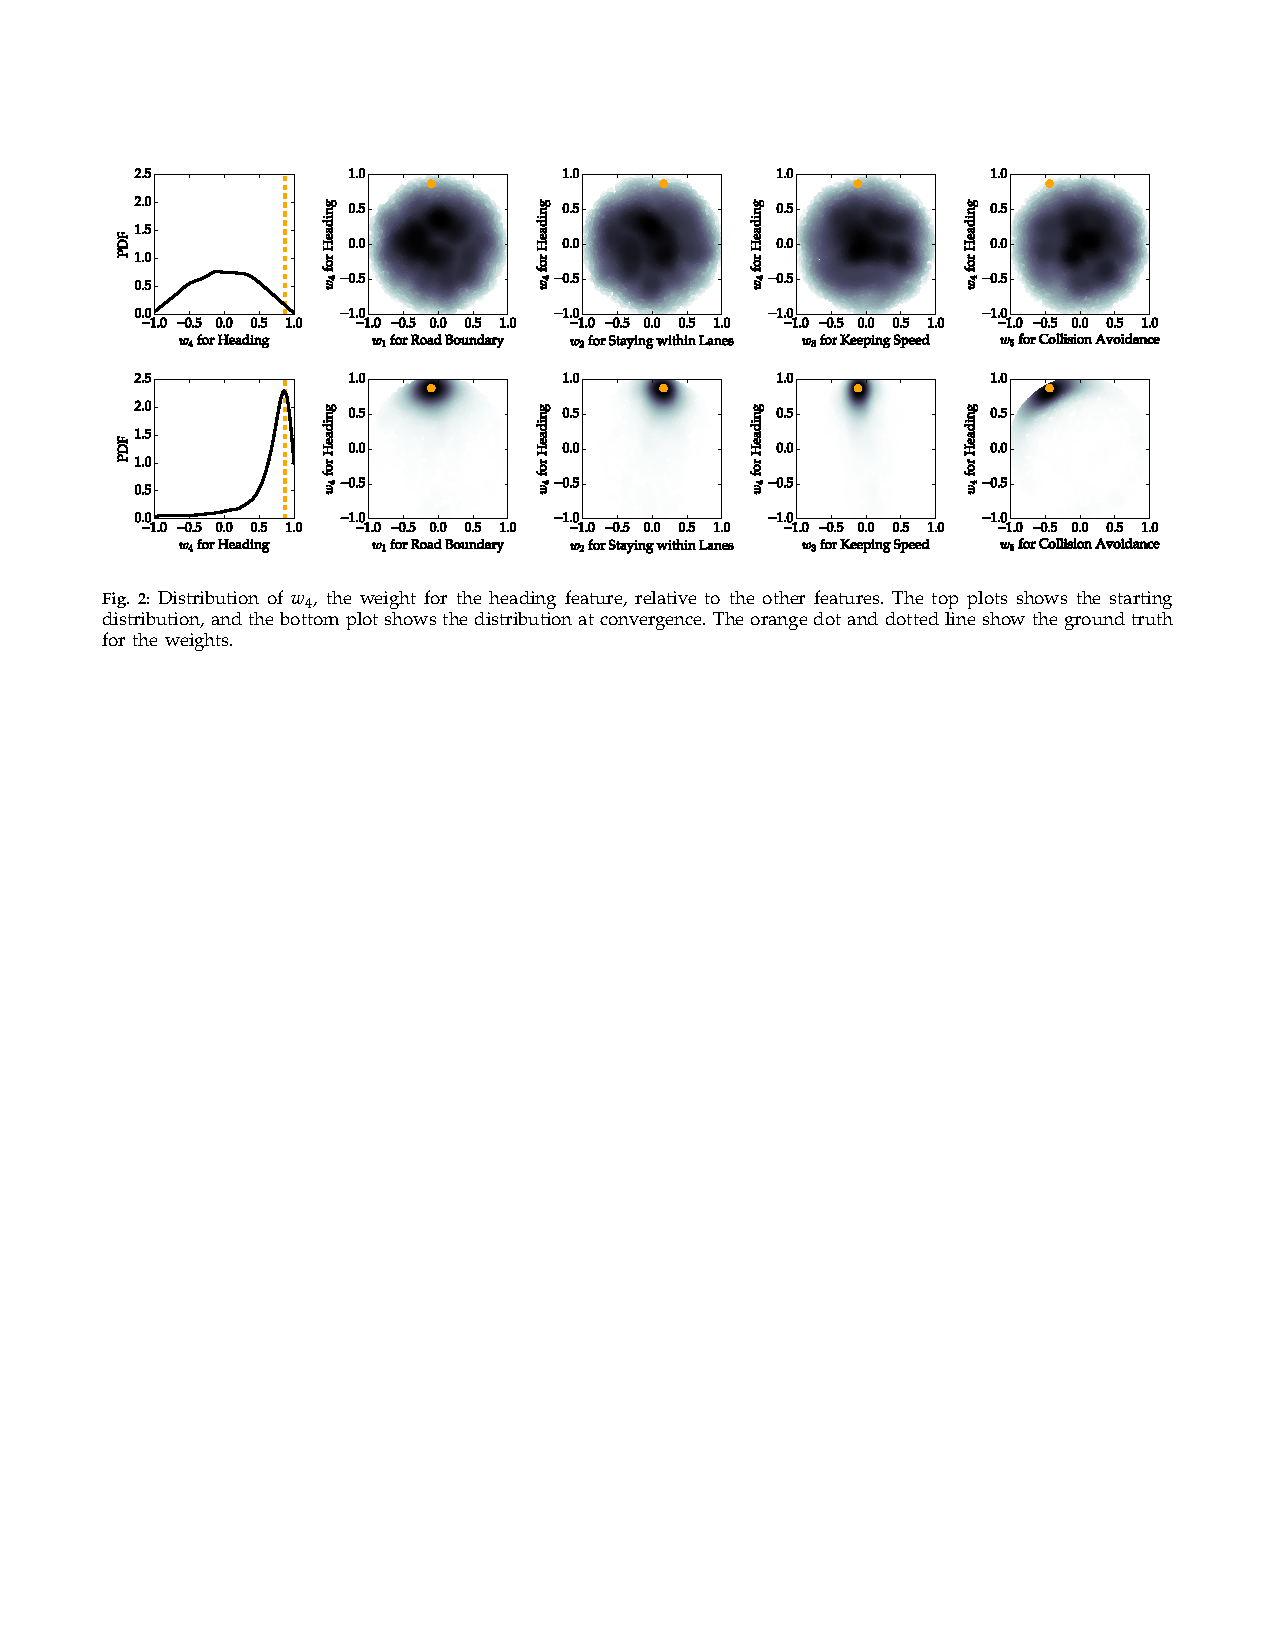
\includegraphics[width = 0.9\textwidth]{./BigResult}
  	\end{center}
  	\begin{center}
  	% \vspace{0.25cm}
  	\includegraphics[width = 0.55\textwidth]{./SmallResult}
  	\end{center}
\end{frame}

\begin{frame}[t]{Discussion}
\begin{itemize} \itemsep 0.05in
	\item What is novel/interesting?
	\begin{itemize} \itemsep 0.025in
		\item \textbf{preference-based} approach allows users to compare two trajectories in various scenarios without having to demonstrate a full trajectory (of how they would like to drive, not how they actually drive)
		\item \textbf{active} enables choosing informative test cases otherwise difficult to encounter in driving scenarios; addresses the limitation of training data sparsity/informativeness
		\item In-depth investigation of the effect of \textbf{synthesis} of real trajectories for dynamical systems compared to relying on a discrete set
	\end{itemize}
	\item Limitations
	\begin{itemize} \itemsep 0.025in
		\item Markov assumption is inherently built into system dynamics
		\item Feature selection is not active/based on expert knowledge
		\item Reward function is constrained to be linear in the feature space
		\item The entire formulation is for a human $H$ with only one other robot $R$
		\item Formulation of $\textbf{w}_{true}$ was unclear
		\item Experiments:
		\begin{itemize} \itemsep 0.025in
			\item potential functions' based reward function
			\item $f_{HR}$ assumed as a simple point mass-dynamics model
		\end{itemize}
	\end{itemize}
\end{itemize}
\end{frame}

\begin{frame}[t]{Questions}
	\begin{center} \Huge Questions? \end{center}
\end{frame}

% Save final frame number, so that backup slides are not counted
\newcounter{finalframe}
\setcounter{finalframe}{\value{framenumber}}

% \begin{frame}[t]{Backup Slide 1}
% 	\begin{itemize} %\itemsep 0.1in
% 		\item Blah blah blah ...
% 	\end{itemize}
% \end{frame}

\begin{frame}[allowframebreaks]{References}
	\tiny
	\def\newblock{}
	\bibliography{IEEEabrv,ref}		% specify bibliography file
									% (ref.bib) here
\end{frame}

\setcounter{framenumber}{\value{finalframe}}
% Set up so that backup slides are not counted in total slides

\end{document}
